\documentclass[11pt,a4paper]{article}

% Standard style with default Computer Modern fonts
\usepackage[margin=1in]{geometry}
\usepackage[T1]{fontenc}
\usepackage[utf8]{inputenc}
\usepackage{amsmath,amssymb,amsthm}
\usepackage{graphicx}
\usepackage{booktabs}
\usepackage{hyperref}
\usepackage{float}
\usepackage{listings}
\usepackage{xcolor}

\hypersetup{
  colorlinks=true,
  linkcolor=blue,
  citecolor=blue,
  urlcolor=blue
}

\lstset{
  basicstyle=\ttfamily\small,
  frame=single,
  breaklines=true,
  showstringspaces=false,
  keywordstyle=\color{blue},
  commentstyle=\color{gray}
}

\title{Probabilistic Demand Forecasting + Stochastic Optimisation for Inventory Control}
\author{Navid Sharifi}
\date{March 21, 2026}

\begin{document}

\maketitle

\begin{abstract}
This article presents an end-to-end route from uncertainty-aware demand forecasting to inventory decisions using stochastic optimisation, robust policy design, and KPI-based evaluation. The core argument is that forecast quality should be judged by operational outcomes, not only by statistical point-error metrics.
\end{abstract}

\section{Introduction}

Forecasting and inventory control are often treated as separate tasks. In practice, this separation is costly. A model with excellent RMSE can still produce poor replenishment decisions if it underestimates tail risk. The right question is not only ``How accurate is my forecast?'' but also ``How much operational cost does my forecast induce?''

This article presents an end-to-end route from probabilistic forecasting to stochastic inventory optimisation. We will:

\begin{enumerate}
    \item Formalise the demand uncertainty problem.
    \item Build probabilistic forecasts rather than point forecasts.
    \item Translate forecast distributions into inventory decisions.
    \item Compare methods on business KPIs, not just forecast error.
\end{enumerate}

Figure~\ref{fig:pipeline} summarizes the full pipeline used throughout this blog.

\begin{figure}[H]
\centering
\fbox{\parbox{0.95\linewidth}{
\centering
\textbf{Figure 1 Pipeline (Flowchart)}\\[4pt]
Raw Demand and Context Data $\rightarrow$ Cleaning and Feature Engineering $\rightarrow$\\
Probabilistic Forecast Model $\rightarrow$ Predictive Distribution and Quantiles $\rightarrow$\\
Scenario Generation $\rightarrow$ Stochastic Inventory Optimisation $\rightarrow$\\
Policy Simulation $\rightarrow$ KPI Dashboard (Cost, Fill Rate, Stockouts) $\rightarrow$\\
Monitoring and Recalibration $\rightarrow$ Feature Engineering (feedback loop)
}}
\caption{End-to-end route from data to inventory decisions.}
\label{fig:pipeline}
\end{figure}

The key idea in Figure~\ref{fig:pipeline} is the feedback loop: forecasting quality and inventory outcomes are evaluated jointly, then used to retrain or recalibrate.

\section{Problem Setup and Notation}

Consider one SKU first, then extend to many SKUs. Let:

\begin{itemize}
    \item $D_{t+h}$ be random demand at forecast origin $t$ and horizon $h$.
    \item $\mathcal{X}_t$ be available information (history, price, promotions, calendar, macro context).
    \item $Q_t$ be order quantity placed at time $t$.
    \item $I_t$ be net inventory position right before demand in period $t$.
\end{itemize}

We forecast a full distribution, not a scalar:

\begin{equation}
D_{t+h} \sim \hat{F}_{t+h}(\cdot \mid \mathcal{X}_t)
\label{eq:forecast_dist}
\end{equation}

where $\hat{F}_{t+h}$ may come from parametric or non-parametric models.

\subsection{Inventory dynamics}

\begin{equation}
I_{t+1} = I_t + Q_t - D_t
\label{eq:inventory_dynamics}
\end{equation}

In settings with lead time $L$, orders affect inventory after $L$ periods. The same state equation applies with delayed receipt terms.

\subsection{Cost structure}

Let $h$ be the holding-cost coefficient, $b$ be backorder or lost-sales penalty coefficient, and $c$ be ordering unit cost. A common multi-period objective is:

\begin{equation}
\min_{\{Q_t\}} \; \mathbb{E}\left[\sum_{t=1}^{T} h(I_t)^+ + b(-I_t)^+ + cQ_t\right]
\label{eq:multi_period_cost}
\end{equation}

subject to capacity, MOQ, lead-time, and service-level constraints.

\section{Forecasting Layer: From Point to Distribution}

\subsection{Why point forecasts are not enough}

Suppose two models have similar MAE. If one underestimates upper-tail demand, stockouts surge when promotions or seasonality shocks occur. Inventory policies are asymmetric: under-forecasting and over-forecasting do not have equal costs.

\subsection{Proper losses for probabilistic forecasts}

For quantile models, use pinball loss:

\begin{equation}
L_{\tau}(y, \hat{q}_{\tau}) = (\tau - \mathbf{1}\{y < \hat{q}_{\tau}\})(y - \hat{q}_{\tau})
\label{eq:pinball}
\end{equation}

For full-distribution models, use proper scoring rules (for example CRPS and log score) to avoid miscalibrated but sharp predictions.

\subsection{Methods to include}

A practical hierarchy:

\begin{enumerate}
    \item Baseline: Croston-family or ETS/ARIMA variants for intermittent or smoother demand.
    \item Deep probabilistic: DeepAR-style autoregressive distribution models.
    \item Interpretable multi-horizon: TFT-style models with static and temporal covariates.
    \item Intermittent-demand deep models: renewal-process formulations for zero-inflated sparse demand.
\end{enumerate}

Figure~\ref{fig:fan_chart} is the minimum visualization that should appear in this section.

\begin{figure}[H]
\centering
\IfFileExists{images/fig2-fan-chart.png}{
  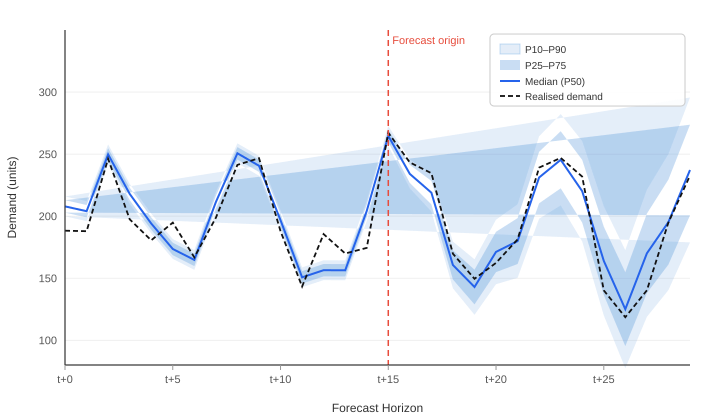
\includegraphics[width=0.88\linewidth]{images/fig2-fan-chart.png}
}{
  \fbox{\parbox{0.88\linewidth}{\centering Placeholder for Figure 2: Quantile fan chart (P10, P50, P90) versus actual demand.}}
}
\caption{Quantile fan chart showing demand uncertainty widening with horizon.}
\label{fig:fan_chart}
\end{figure}

Interpretation of Figure~\ref{fig:fan_chart}:

\begin{itemize}
    \item If actuals frequently fall outside P10--P90, uncertainty is underestimated.
    \item If intervals are too wide, safety stock will be inflated and holding costs will rise.
\end{itemize}

\begin{figure}[H]
\centering
\IfFileExists{images/fig3-calibration-curve.png}{
  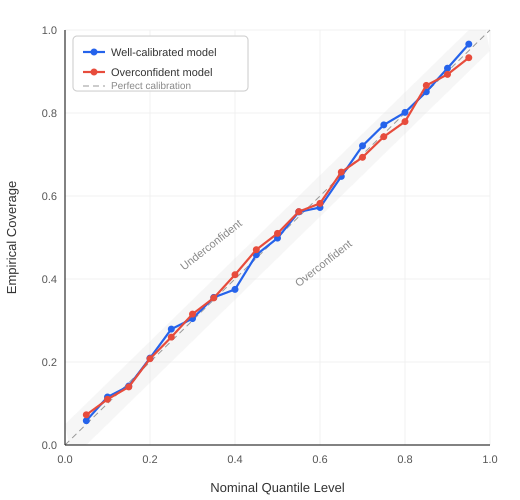
\includegraphics[width=0.82\linewidth]{images/fig3-calibration-curve.png}
}{
  \fbox{\parbox{0.82\linewidth}{\centering Placeholder for Figure 3: Calibration curve (predicted quantile level vs empirical coverage).}}
}
\caption{Predicted quantile level versus empirical coverage. The diagonal is ideal calibration.}
\label{fig:calibration}
\end{figure}

Figure~\ref{fig:calibration} checks whether nominal quantiles match realized frequencies. For example, the 0.9 quantile should be exceeded about 10\% of the time.

\section{Decision Layer: Stochastic Inventory Optimisation}

\subsection{Single-period newsvendor intuition}

Let underage cost be $c_u$ and overage cost be $c_o$. The expected single-period cost is:

\begin{equation}
\min_q \; \mathbb{E}\left[c_o(q-D)^+ + c_u(D-q)^+\right]
\label{eq:newsvendor}
\end{equation}

The optimal order-up-to level is the critical fractile:

\begin{equation}
q^* = F_D^{-1}\left(\frac{c_u}{c_u + c_o}\right)
\label{eq:critical_fractile}
\end{equation}

Equation~\eqref{eq:critical_fractile} directly links statistical output to business preference. High stockout penalty relative to holding cost pushes the chosen quantile upward.

\subsection{Multi-period scenario-based optimisation}

For realistic operations, sample scenarios from $\hat{F}$ and optimize against expected cost under those paths. Let scenario index be $s=1,\dots,S$ with probability $p_s$.

\begin{equation}
\min_{\{Q_t\}} \; \sum_{s=1}^{S} p_s \sum_{t=1}^{T}\left[h(I_{t,s})^+ + b(-I_{t,s})^+ + cQ_t\right]
\label{eq:scenario_program}
\end{equation}

subject to inventory transitions per scenario and operational constraints.

\subsection{Distributionally robust extension}

Forecast errors and regime shifts make pure stochastic programs fragile. One robust alternative is to optimize worst-case expected cost over an ambiguity set $\mathcal{P}$ around the nominal demand law:

\begin{equation}
\min_{\pi \in \Pi} \; \sup_{\mathbb{P} \in \mathcal{P}} \mathbb{E}_{\mathbb{P}}\big[C(\pi, D)\big]
\label{eq:dro}
\end{equation}

where $\pi$ is a policy (for example base-stock policy). Equation~\eqref{eq:dro} is useful when demand exhibits structural breaks.

\begin{figure}[H]
\centering
\IfFileExists{images/fig4-cost-service-frontier.png}{
  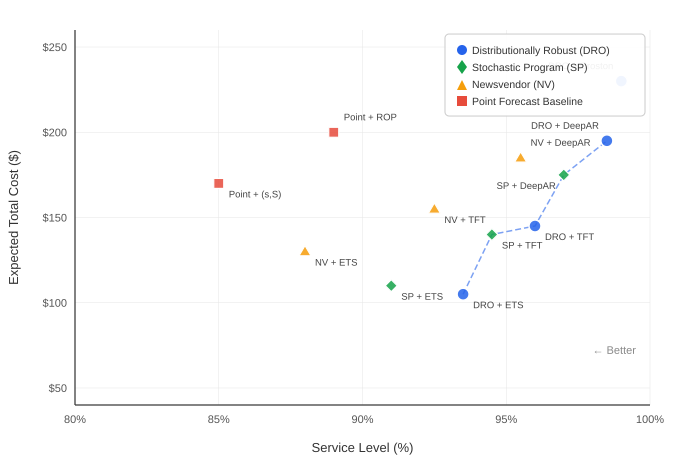
\includegraphics[width=0.86\linewidth]{images/fig4-cost-service-frontier.png}
}{
  \fbox{\parbox{0.86\linewidth}{\centering Placeholder for Figure 4: Cost-service frontier across policy-model combinations.}}
}
\caption{Pareto frontier of service level versus total expected cost.}
\label{fig:frontier}
\end{figure}

Figure~\ref{fig:frontier} visualizes the service-cost trade-off from competing policies.

\section{Experiment Design for a Credible Study}

To make this post technically strong, evaluate forecasting and control jointly.

\subsection{Backtesting protocol}

\begin{enumerate}
    \item Use rolling-origin evaluation (multiple forecast origins).
    \item Keep training windows and horizon fixed, or explicitly report expanding-window logic.
    \item Refit or update models with a realistic cadence.
\end{enumerate}

\subsection{Scenario generation}

At each origin, draw $S$ demand paths from the predictive distribution over the lead-time and planning horizon. Use these paths in Equation~\eqref{eq:scenario_program}.

\subsection{KPI set}

Forecast KPIs:
\begin{itemize}
    \item Pinball loss across quantiles
    \item CRPS
    \item Coverage error at key quantiles
\end{itemize}

Inventory KPIs:
\begin{itemize}
    \item Total cost
    \item Fill rate
    \item Stockout frequency
    \item Average on-hand inventory
    \item Cost volatility across scenarios
\end{itemize}

\begin{figure}[H]
\centering
\IfFileExists{images/fig5-kpi-boxplots.png}{
  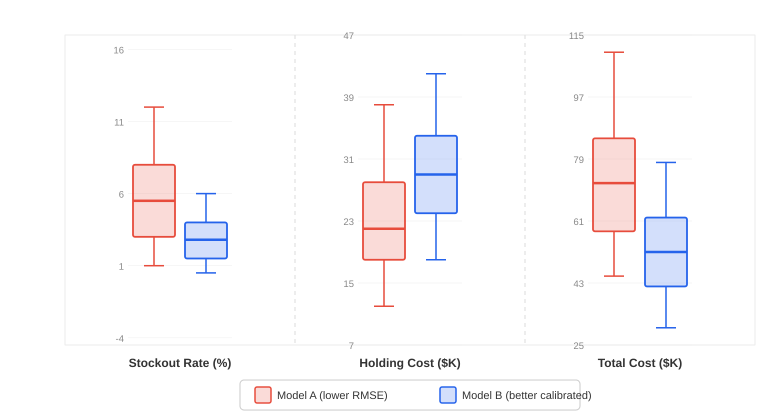
\includegraphics[width=0.88\linewidth]{images/fig5-kpi-boxplots.png}
}{
  \fbox{\parbox{0.88\linewidth}{\centering Placeholder for Figure 5: KPI boxplots from Monte Carlo simulation.}}
}
\caption{Distribution of stockout rate, holding cost, and total cost by method.}
\label{fig:kpi_boxplots}
\end{figure}

Figure~\ref{fig:kpi_boxplots} compares policy outcomes under simulation.

\section{Why Forecast Accuracy and Inventory Cost Diverge}

Suppose Model A has lower RMSE than Model B but poorer calibration near upper quantiles. Under service targets, Model A can still yield higher total cost because it triggers frequent shortage penalties. This is the practical lesson:

\begin{itemize}
    \item Point error metrics compress asymmetric business consequences.
    \item Decision-aware evaluation preserves asymmetry through cost structure.
\end{itemize}

A robust study should explicitly report cases where ranking by RMSE conflicts with ranking by total inventory cost.

\section{Implementation Blueprint}

\subsection*{Step 1: Data and feature engineering}
\begin{itemize}
    \item Include promotions, holidays, price, and stockout flags.
    \item Separate true zero demand from censored demand caused by stockouts.
\end{itemize}

\subsection*{Step 2: Probabilistic model training}
\begin{itemize}
    \item Train at least one statistical baseline and one deep probabilistic model.
    \item Tune for probabilistic objectives (Equation~\eqref{eq:pinball}, CRPS), not only MAE.
\end{itemize}

\subsection*{Step 3: Calibration checks}
\begin{itemize}
    \item Produce fan chart (Figure~\ref{fig:fan_chart}) and calibration plot (Figure~\ref{fig:calibration}).
    \item Recalibrate quantiles if systematic bias appears.
\end{itemize}

\subsection*{Step 4: Optimisation}
\begin{itemize}
    \item Convert calibrated distributions to ordering decisions via Equations~\eqref{eq:critical_fractile} and \eqref{eq:scenario_program}.
    \item Add robust variant via Equation~\eqref{eq:dro} for stress testing.
\end{itemize}

\subsection*{Step 5: Simulation and decision report}
\begin{itemize}
    \item Simulate policies over historical rolling windows.
    \item Plot Figure~\ref{fig:frontier} and Figure~\ref{fig:kpi_boxplots}.
    \item Select policy by expected cost plus risk tolerance.
\end{itemize}

\section{Reproducible Pseudocode}

\begin{lstlisting}[language=Python]
# 1) fit probabilistic model
model.fit(train_data)

# 2) generate quantiles or full predictive distribution
pred_dist = model.predict_distribution(features_test)

# 3) scenario sampling for planning horizon
scenarios = pred_dist.sample(num_scenarios=1000)

# 4) solve stochastic inventory optimization
policy = optimize_inventory(
    scenarios,
    holding_cost=h,
    shortage_cost=b,
    order_cost=c,
    constraints=ops_constraints,
)

# 5) forward simulation and KPI tracking
results = simulate_policy(policy, realized_demand)
report_kpis(results)
\end{lstlisting}

This pseudocode maps directly to the pipeline in Figure~\ref{fig:pipeline}.

\section{Practical Pitfalls and How to Avoid Them}

\begin{enumerate}
    \item Leakage in feature engineering: use only information known at forecast origin.
    \item Ignoring stockout censorship: observed sales are not always true demand.
    \item Evaluating forecasts without operations: always include policy simulation and business KPIs.
    \item Overfitting quantile models: cross-validate and check calibration on holdout horizons.
    \item No stress testing: evaluate performance under demand shocks and lead-time variability.
\end{enumerate}

\section{References and Reading Route}

\begin{enumerate}
    \item Flunkert, Salinas, Gasthaus. \textit{DeepAR: Probabilistic Forecasting with Autoregressive Recurrent Networks}. arXiv:1704.04110.
    \item Lim, Arik, Loeff, Pfister. \textit{Temporal Fusion Transformers for Interpretable Multi-horizon Time Series Forecasting}. arXiv:1912.09363.
    \item Oreshkin et al. \textit{N-BEATS: Neural Basis Expansion Analysis for Time Series Forecasting}. arXiv:1905.10437.
    \item Turkmen, Wang. \textit{Intermittent Demand Forecasting with Deep Renewal Processes}. arXiv:1911.10416.
    \item Ozer et al. \textit{Combining Probabilistic Forecasts of Intermittent Demand}. arXiv:2304.03092.
    \item Bertsimas et al. \textit{Distributionally Robust Newsvendor with Moment Constraints}. arXiv:2010.16369.
    \item Natarajan et al. \textit{On the Heavy-tail Behavior of the Distributionally Robust Newsvendor}. arXiv:1806.05379.
    \item Recent decision-centric preprints on forecast-to-inventory KPI alignment (2023--2026).
\end{enumerate}

Include peer-reviewed journal versions where available, and label preprints explicitly as preprints.

\section{Conclusion}

The central message is simple: forecast uncertainty is only useful when it changes decisions.

Equations~\eqref{eq:forecast_dist} to \eqref{eq:pinball} define how to model and evaluate uncertainty. Equations~\eqref{eq:newsvendor} to \eqref{eq:dro} define how to convert uncertainty into robust inventory actions. Figures~\ref{fig:pipeline} to \ref{fig:kpi_boxplots} show how to operationalize and validate the full route.

If final model selection is based on expected inventory cost and service reliability rather than only RMSE, demand forecasting is aligned with real operational goals.

\appendix
\section{Suggested Figure Asset Names}

To keep your repository organized, store chart images with these names:

\begin{itemize}
    \item \texttt{images/fig2-fan-chart.png}
    \item \texttt{images/fig3-calibration-curve.png}
    \item \texttt{images/fig4-cost-service-frontier.png}
    \item \texttt{images/fig5-kpi-boxplots.png}
\end{itemize}

Then Figure 2 to Figure 5 will render automatically when assets are present.

\end{document}
